%================================================================
% This software is free: you can redistribute it and/or modify it %
% under the terms of the GNU General Public License Version 3, as %
% as published by the Free Software Foundation.                   %
% This software is distributed in the hope that it will be useful,%
% but WITHOUT ANY WARRANTY; without even the implied warranty of  %
% MERCHANTABILITY or FITNESS FOR A PARTICULAR PURPOSE. See the    %
% GNU General Public License for more details.                    %
% You should have received a copy of the GNU General Public		  %
% License Version 3 in the file COPYING that came with this       %
% distribution.     										      %
%If not, see <http://www.gnu.org/licenses/>                       %
% =============================================================== %
%                                                                 %
% Copyright (c) 2017 Grupo de Estudio y Desarrollo en Rob�tica    %  
% Universidad Santo Tom�s - Bogot�, Colombia                      %
% http://www.stoxs.org/                                           %
%                                                                 %
% =============================================================== %
\documentclass[12pt]{article}

% ======================== Pre�mbulo ======================== %
%Paquetes
%\usepackage[letterpaper, left=3cm, top=3.0cm,right=3cm,bottom=5.5cm,showframe,headsep=0.5cm,headheight=3cm]{geometry}
\usepackage[letterpaper, left=3cm, top=3.0cm,right=3cm,bottom=5.5cm,headsep=0.8	cm,headheight=3cm]{geometry}
\usepackage[spanish]{babel}
\usepackage[latin5]{inputenc}
\usepackage{graphicx}
\usepackage{amssymb,amsmath}
\usepackage{fancyhdr}
\usepackage{titlesec}
\usepackage{standalone}
\usepackage{multirow}

%Formato
\pagestyle{fancy}
\titleformat{\section}
{\normalfont\fontsize{14}{15}\bfseries}{\thesection}{1em}{}
\titleformat{\subsection}
{\normalfont\fontsize{13}{15}\bfseries}{\thesubsection}{1em}{}
\renewcommand\refname{Bibliograf�a}
\graphicspath{ {img/} }

%Encabezados y pie de p�gina
\fancyhead[]{}
\chead{
\includegraphics[width=8.5cm]{img/SantoTomasHeader.png}}
\cfoot{
\includegraphics[width=0.9\textwidth]{img/SantoTomasFooter.png}}
\renewcommand{\headrulewidth}{0pt}
\pagestyle{fancyplain}

% ======================== Documento ======================== %
\begin{document}
\begin{titlepage}
	%Portada
	\centering
		{\scshape\LARGE Universidad Santo Tom�s \par}
		\vspace{0.2cm}
		{\scshape\Large Facultad de Ingenier�a Electr�nica \par}
		\vspace{1.5cm}
		
\includegraphics[width=0.3\textwidth]{GED_LOGO}\par\vspace{1cm}
		\vspace{0.5cm}
		{\huge\bfseries ``T�tulo del proyecto FODEIN 2018''\par}
		\vspace{1cm}
		{\Large\itshape Nombre de los Autores \par}
		\vfill
		% Bottom of the page
		{\large 11 de septiembre de 2017\par}
	\end{titlepage}
	
	%Secciones del documento
	\documentclass{standalone}
\usepackage[spanish]{babel}   %%para Colocar en Espanol
\usepackage[latin5]{inputenc} %%para usar tildes adecuadamente
\begin{document}

\section*{T�tulo}
T�tulo de la propuesta FODEIN

\section*{Duraci�n}
Duraci�n (en meses)

\section*{Lugar de ejecuci�n}
Lugar de ejecuci�n

\section*{Investigador principal}
Investigador principal

\section*{Co-investigador(es)}
Co-investigador(es)

{\small
\begin{tabular}{llllll}
	\hline
	\multicolumn{6}{|c|}{\textbf{Datos generales}}                                                                                                                                                                                                                                                                                                                                                                                                                                                                                                                                                                                                                                                                                                                                                                                                                                                             \\ \hline
	\multicolumn{1}{|c|}{\textbf{Programa}}& \multicolumn{1}{c|}{\textbf{Facultad}}&                                   \multicolumn{1}{c|}{\begin{tabular}[c]{@{}c@{}}
			\textbf{L�nea}\\ \textbf{activa}\end{tabular}}& \multicolumn{1}{c|}{\begin{tabular}[c]{@{}c@{}}
			\textbf{L�nea}\\ \textbf{medular}\end{tabular}}& \multicolumn{1}{c|}{\begin{tabular}[c]{@{}c@{}}
			\textbf{Campos de acci�n}\\ \textbf{institucional}\end{tabular}}&                                          \multicolumn{1}{c|}{\begin{tabular}[c]{@{}c@{}}
			\textbf{Grupo de}\\ \textbf{investigaci�n}\end{tabular}} \\ \hline
	\multicolumn{1}{|l|}{\begin{tabular}[c]{@{}l@{}}
			Ingenieri�a\\Electr�nica\end{tabular}}& \multicolumn{1}{l|}{\begin{tabular}[c]{@{}l@{}}
			Ingenieri�a\\Electr�nica\end{tabular}}& \multicolumn{1}{l|}{\begin{tabular}[c]{@{}l@{}}
			Inteligencia\\Computacional\end{tabular}}& \multicolumn{1}{l|}{\begin{tabular}[c]{@{}l@{}}
			Alberto\\ Magno\end{tabular}}& \multicolumn{1}{l|}{\begin{tabular}[c]{@{}l@{}}
			Derechos humanos,\\ ciudadan�a y \\ construcci�n de \\ pol�tica p�blica en \\ y para escenarios de \\ paz (  )\\ \\ Desarrollo tecnol�gico \\ con apuesta social (X)\\ \\ Desarrollo ambiental \\ sostenible( )\\ \\ Cambio educativo y \\ social desde la multi \\ e interculturalidad ( )\end{tabular}}& \multicolumn{1}{l|}{\begin{tabular}[c]{@{}l@{}}
			Grupo de\\Estudio y\\Desarrollo en\\Rob�tica\\GED\end{tabular}} \\ \hline
\end{tabular}
}

\section*{Equipo de investigaci�n requerido}
Enuncie el n�mero de investigadores, si son egresados, profesionales externos, auxiliares, asistentes, con su respectivo nivel de formaci�n, o si se vincular� un semillero de investigaci�n

\section*{Alianza estrat�gica}
Mencione si el proyecto se presenta en colaboraci�n con otras instituciones, enuncie el nombre de las instituciones

\section*{Resumen de la propuesta}
M�ximo 300 palabras

\section*{Palabras Clave}
M�ximo 5 palabras

\end{document}
	\documentclass{standalone}
\usepackage[spanish]{babel}   %%para Colocar en Español
\usepackage[latin5]{inputenc} %%para usar tildes adecuadamente
\begin{document}
	\section*{Planteamiento del problema y pregunta de investigaci\'on}
	Planteamiento del problema y pregunta de investigaci\'on

\end{document}
	\documentclass{standalone}
\usepackage[spanish]{babel}   %%para Colocar en Español
\usepackage[latin5]{inputenc} %%para usar tildes adecuadamente
\begin{document}
\section*{Justificaci\'on}
Justificaci\'on

\end{document}
	\documentclass{standalone}
\usepackage[spanish]{babel}   %%para Colocar en Español
\usepackage[latin5]{inputenc} %%para usar tildes adecuadamente
\begin{document}
	\section*{Objetivo general}
	Objetivo general
	
	\section*{Objetivos espec\'ificos}
	Objetivos espec\'ificos

\end{document}
	\documentclass{standalone}
\usepackage[spanish]{babel}   %%para Colocar en Español
\usepackage[latin5]{inputenc} %%para usar tildes adecuadamente

\begin{document}
	\section*{Marco te\'orico}
	Ejemplo para realizar citaciones dentro del documento: Se pueden citar referencias individuales \cite{murphy} o tambi�n se pueden citar m�ltiples referencias \cite{murphy,matlab}. 
	
	Ejemplo para usar figuras: En la Figura \ref{fig:stoxs_2016} se observan  3 robots del equipo STOx's en partido oficial de RoboCup 2016.
	
	\begin{figure}
		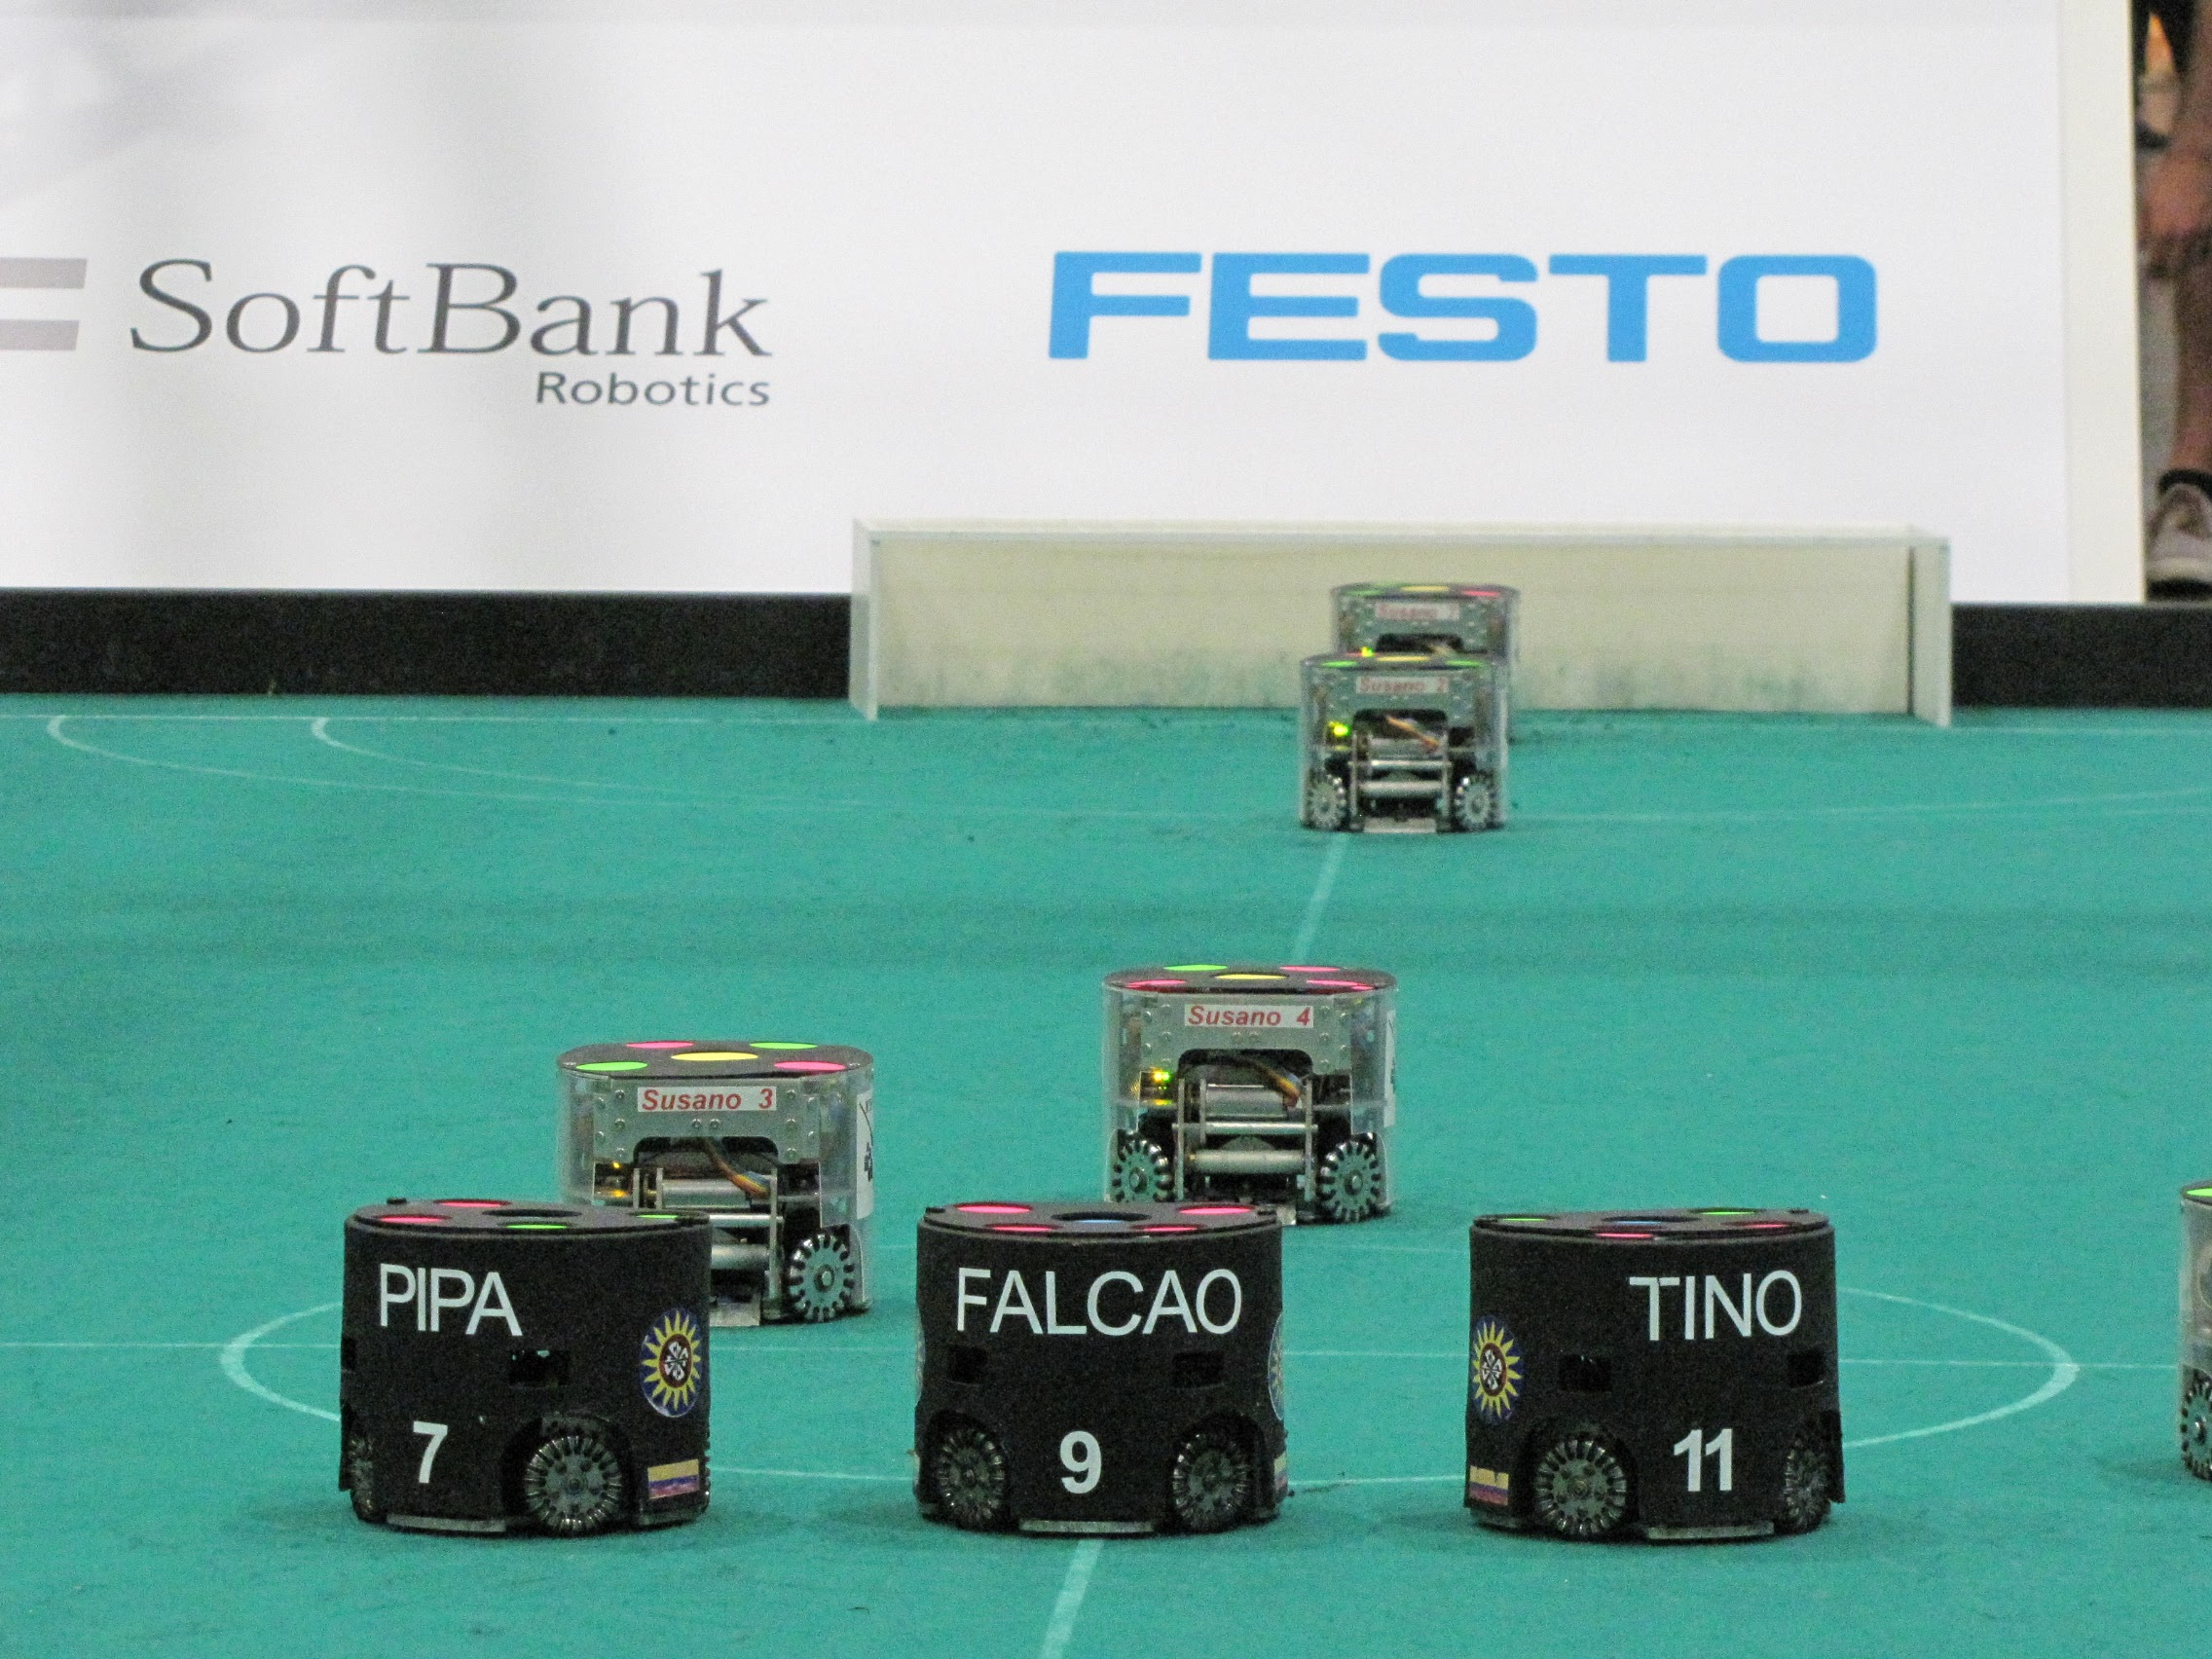
\includegraphics[width=\textwidth]{STOxs.jpg}
		\caption{Robots del equipo STOx's en RoboCup 2016}
		\label{fig:stoxs_2016}
	\end{figure}

\end{document}
	\documentclass{standalone}
\usepackage[spanish]{babel}   %%para Colocar en Español
\usepackage[latin5]{inputenc} %%para usar tildes adecuadamente
\begin{document}
	\section*{Metodolog\'ia}
	Metodolog\'ia

\end{document}
	\documentclass{standalone}
\usepackage[spanish]{babel}   %%para Colocar en Español
\usepackage[latin5]{inputenc} %%para usar tildes adecuadamente
\begin{document}
	\section*{Resultados esperados}
	Resultados esperados
	
	\section*{Productos esperados}
	Relaci�nelos de acuerdo con la tipolog�a de Colciencias- Ver Tabla anexa a la convocatoria
	
	\section*{Contribuci�n del proyecto al cumplimiento de la misi�n institucional}
	 Se pueden consultar en la p�gina de la Unidad de Investigaci�n
	 \begin{enumerate}
	 	\item Con qu� l�neas del PIM se vincula el proyecto:
	 	\item Con qu� acciones del Plan General de Desarrollo Bogot�, se articula el proyecto:
	 \end{enumerate}	
\end{document}
	\documentclass{standalone}
\usepackage[spanish]{babel}   %%para Colocar en Espa�ol
\usepackage[latin5]{inputenc} %%para usar tildes adecuadamente
\usepackage{multirow}

\begin{document}
	\section*{Presupuesto}
		\small
\begin{tabular}{|l|l|l|}\hline
\multicolumn{3}{|c|}{\textbf{Recurso solicitado FODEIN}}\\ \hline
\multicolumn{1}{|c|}{\textbf{Concepto}}& \multicolumn{1}{c|}{\textbf{Descripci\'on}}& \multicolumn{1}{c|}{\textbf{Monto}} \\ \hline
\multirow{3}{*}{Personal cient\'ifico}&
Nombre del docente 1 & \$10'000.000  \\ \cline{2-3}&
Nombre del docente 2 & \$10'000.000  \\ \cline{2-3}& 
Nombre del docente 3 & \$10'000.000  \\ \hline
Auxilio a investigadores& 
\begin{tabular}[c]{@{}l@{}}Reconocimiento econ\'omico \\ 
a estudiantes de pregrado\end{tabular}& \$10'000.000  \\ \hline
Asistentes de investigaci\'on & 
\begin{tabular}[c]{@{}l@{}}Reconocimiento econ\'omico \\ 
a estudiantes de posgrado\end{tabular}& \$10'000.000  \\ \hline
Equipos & 
\begin{tabular}[c]{@{}l@{}}Consultar en adquisiciones y \\ 
suministros para evitar duplicidad\end{tabular}& \$10'000.000   \\ \hline
Software &
\begin{tabular}[c]{@{}l@{}}Consultar en departamento TICS\\ 
para evitar duplicidad\end{tabular}& \$10'000.000   \\ \hline
Materiales &
\begin{tabular}[c]{@{}l@{}}Descripci\'on muy corta de los\\ 
materiales que se piensan utilizar\end{tabular}& \$10'000.000 \\ \hline
Papeler\'ia & 
\begin{tabular}[c]{@{}l@{}}Descripci\'on muy corta de la\\ 
papeleria que se piensan utilizar\end{tabular}& \$10'000.000 \\ \hline
Fotocopias & 
\begin{tabular}[c]{@{}l@{}}Descripci\'on \\ 
Fotocopias\end{tabular}& \$10'000.000  \\ \hline
Salidas de campo & 
\begin{tabular}[c]{@{}l@{}}Lugar, tiempos, actividades, \\ 
investigadores\end{tabular}& \$10'000.000 \\ \hline
Material bibliogr\'afico & 
\begin{tabular}[c]{@{}l@{}}Libros, suscripciones a \\
revistas,etc\end{tabular}& \$10'000.000   \\ \hline
Publicaciones & 
\begin{tabular}[c]{@{}l@{}}Libros, traducciones publicaci\'on en \\
revistas\end{tabular}& \$10'000.000 \\ \hline
Servicios t\'ecnicos & 
\begin{tabular}[c]{@{}l@{}}Laboratorios, \\
personas naturales\end{tabular}& \$10'000.000 \\ \hline
Movilidad acad\'emica & 
\begin{tabular}[c]{@{}l@{}}Eventos para socializaci\'on de \\ 
avances y resultados, pasant\'ias\end{tabular} & \$10'000.000 \\ \hline
Organizaci\'on de eventos & 
\begin{tabular}[c]{@{}l@{}}Eventos para difusi\'on de\\ 
resultados \end{tabular}& \$10'000.000 \\ \hline
& 
Total & \$10'000.000                        \\ \hline
\multicolumn{3}{|c|}{\textbf{Contrapartida externa}}                                                                                                                                              \\
\multicolumn{3}{|c|}{Para proyectos en cooperaci\'on y alianza estrat\'egica}                                                                                                                     \\ \hline
\multicolumn{1}{|c|}{\textbf{Instituci\'on}} & \multicolumn{1}{c|}{\textbf{Descripci\'on}}  & \multicolumn{1}{c|}{\textbf{Monto}} \\ \hline& 
Detalle los montos y los conceptos & \\ \hline&                                                                                                              &\\ \hline
& Total                                                                                                        &\\ \hline
\end{tabular}

				
	
	\section*{Cronograma}
	Cronograma

\end{document}
	\documentclass{standalone}
\usepackage[spanish]{babel}   %%para Colocar en Español
\usepackage[latin5]{inputenc} %%para usar tildes adecuadamente

\begin{document}
\bibliography{bib/bibFile}
\bibliographystyle{IEEEtran}
\end{document}

	\documentclass{standalone}
\usepackage[spanish]{babel}   %%para Colocar en Español
\usepackage[latin5]{inputenc} %%para usar tildes adecuadamente
\begin{document}
	\section*{Posibles evaluadores}
	Lista de posibles evaluadores

\end{document}
\end{document}
% ========================== Fin ========================== %